% Created by tikzDevice version 0.12.3.1 on 2022-08-29 14:39:49
% !TEX encoding = UTF-8 Unicode
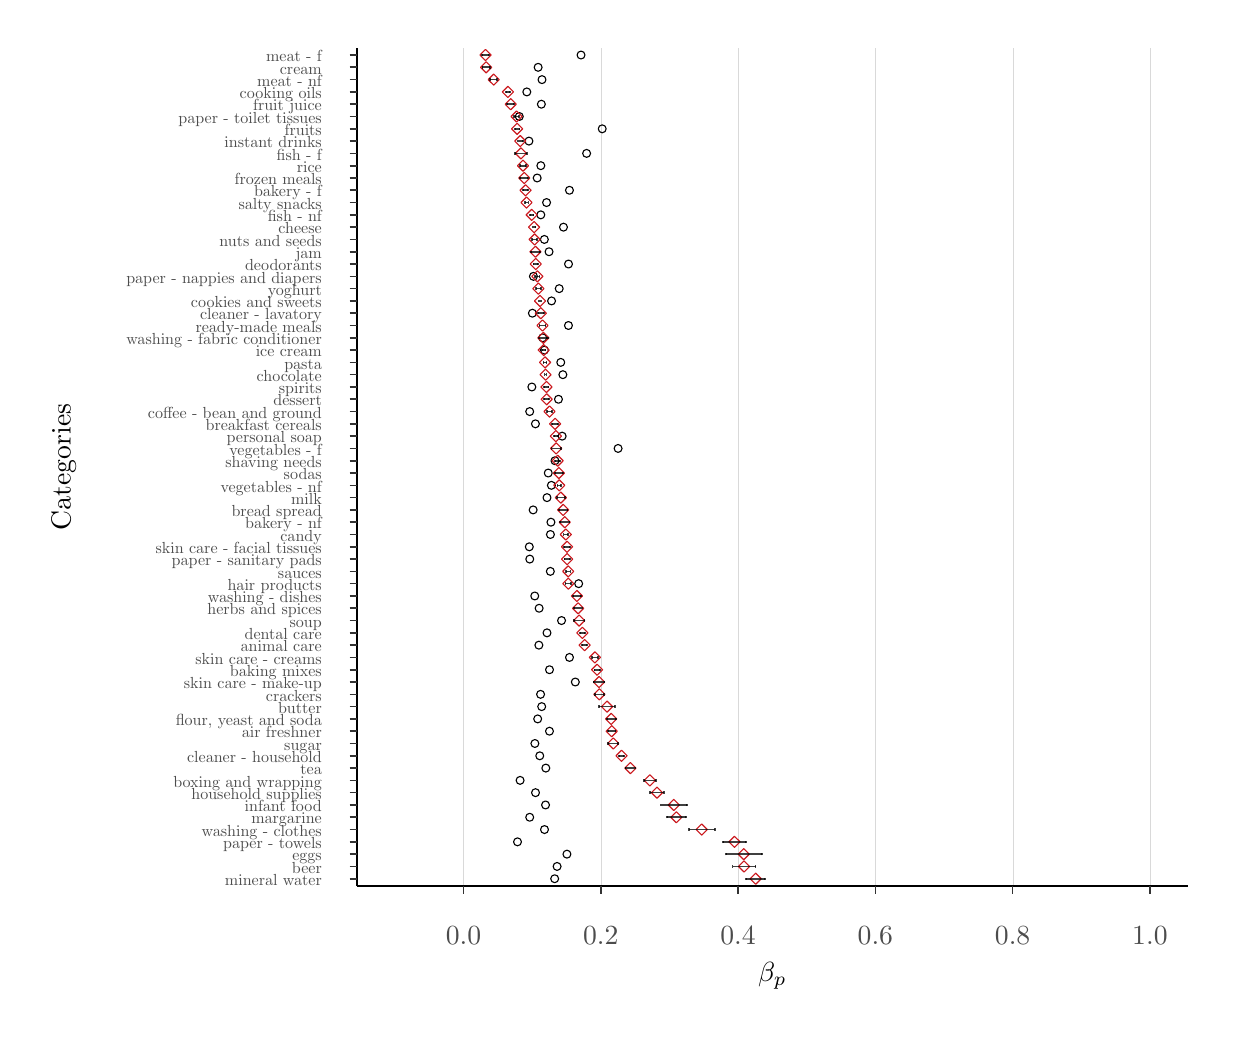
\begin{tikzpicture}[x=1pt,y=1pt]
\definecolor{fillColor}{RGB}{255,255,255}
\path[use as bounding box,fill=fillColor,fill opacity=0.00] (0,0) rectangle (433.62,361.35);
\begin{scope}
\path[clip] (  0.00,  0.00) rectangle (433.62,361.35);
\definecolor{drawColor}{RGB}{255,255,255}
\definecolor{fillColor}{RGB}{255,255,255}

\path[draw=drawColor,line width= 0.6pt,line join=round,line cap=round,fill=fillColor] (  0.00,  0.00) rectangle (433.62,361.35);
\end{scope}
\begin{scope}
\path[clip] (119.04, 51.15) rectangle (419.17,354.12);
\definecolor{drawColor}{RGB}{255,255,255}

\path[draw=drawColor,line width= 0.3pt,line join=round] (132.68, 51.15) --
	(132.68,354.12);

\path[draw=drawColor,line width= 0.3pt,line join=round] (182.29, 51.15) --
	(182.29,354.12);

\path[draw=drawColor,line width= 0.3pt,line join=round] (231.90, 51.15) --
	(231.90,354.12);

\path[draw=drawColor,line width= 0.3pt,line join=round] (281.51, 51.15) --
	(281.51,354.12);

\path[draw=drawColor,line width= 0.3pt,line join=round] (331.11, 51.15) --
	(331.11,354.12);

\path[draw=drawColor,line width= 0.3pt,line join=round] (380.72, 51.15) --
	(380.72,354.12);
\definecolor{drawColor}{gray}{0.85}

\path[draw=drawColor,line width= 0.1pt,line join=round] (157.49, 51.15) --
	(157.49,354.12);

\path[draw=drawColor,line width= 0.1pt,line join=round] (207.09, 51.15) --
	(207.09,354.12);

\path[draw=drawColor,line width= 0.1pt,line join=round] (256.70, 51.15) --
	(256.70,354.12);

\path[draw=drawColor,line width= 0.1pt,line join=round] (306.31, 51.15) --
	(306.31,354.12);

\path[draw=drawColor,line width= 0.1pt,line join=round] (355.92, 51.15) --
	(355.92,354.12);

\path[draw=drawColor,line width= 0.1pt,line join=round] (405.52, 51.15) --
	(405.52,354.12);
\definecolor{drawColor}{RGB}{0,0,0}

\path[draw=drawColor,line width= 0.4pt,line join=round,line cap=round] (192.07,267.05) circle (  1.43);

\path[draw=drawColor,line width= 0.4pt,line join=round,line cap=round] (186.11,249.28) circle (  1.43);

\path[draw=drawColor,line width= 0.4pt,line join=round,line cap=round] (183.23,155.99) circle (  1.43);

\path[draw=drawColor,line width= 0.4pt,line join=round,line cap=round] (186.75, 71.59) circle (  1.43);

\path[draw=drawColor,line width= 0.4pt,line join=round,line cap=round] (189.24,195.97) circle (  1.43);

\path[draw=drawColor,line width= 0.4pt,line join=round,line cap=round] (213.34,209.30) circle (  1.43);

\path[draw=drawColor,line width= 0.4pt,line join=round,line cap=round] (187.23, 93.80) circle (  1.43);

\path[draw=drawColor,line width= 0.4pt,line join=round,line cap=round] (183.28,102.69) circle (  1.43);

\path[draw=drawColor,line width= 0.4pt,line join=round,line cap=round] (182.18,231.51) circle (  1.43);

\path[draw=drawColor,line width= 0.4pt,line join=round,line cap=round] (192.91,147.11) circle (  1.43);

\path[draw=drawColor,line width= 0.4pt,line join=round,line cap=round] (188.11,200.42) circle (  1.43);

\path[draw=drawColor,line width= 0.4pt,line join=round,line cap=round] (197.89,124.90) circle (  1.43);

\path[draw=drawColor,line width= 0.4pt,line join=round,line cap=round] (181.26,173.76) circle (  1.43);

\path[draw=drawColor,line width= 0.4pt,line join=round,line cap=round] (195.78,133.78) circle (  1.43);

\path[draw=drawColor,line width= 0.4pt,line join=round,line cap=round] (190.54,204.86) circle (  1.43);

\path[draw=drawColor,line width= 0.4pt,line join=round,line cap=round] (188.86,164.88) circle (  1.43);

\path[draw=drawColor,line width= 0.4pt,line join=round,line cap=round] (187.50,298.15) circle (  1.43);

\path[draw=drawColor,line width= 0.4pt,line join=round,line cap=round] (185.43,311.48) circle (  1.43);

\path[draw=drawColor,line width= 0.4pt,line join=round,line cap=round] (195.41,253.73) circle (  1.43);

\path[draw=drawColor,line width= 0.4pt,line join=round,line cap=round] (193.13,213.74) circle (  1.43);

\path[draw=drawColor,line width= 0.4pt,line join=round,line cap=round] (192.63,240.40) circle (  1.43);

\path[draw=drawColor,line width= 0.4pt,line join=round,line cap=round] (177.00, 67.15) circle (  1.43);

\path[draw=drawColor,line width= 0.4pt,line join=round,line cap=round] (177.64,329.25) circle (  1.43);

\path[draw=drawColor,line width= 0.4pt,line join=round,line cap=round] (181.43,169.32) circle (  1.43);

\path[draw=drawColor,line width= 0.4pt,line join=round,line cap=round] (182.75,271.49) circle (  1.43);

\path[draw=drawColor,line width= 0.4pt,line join=round,line cap=round] (186.70,284.82) circle (  1.43);

\path[draw=drawColor,line width= 0.4pt,line join=round,line cap=round] (190.43, 53.82) circle (  1.43);

\path[draw=drawColor,line width= 0.4pt,line join=round,line cap=round] (187.65,191.53) circle (  1.43);

\path[draw=drawColor,line width= 0.4pt,line join=round,line cap=round] (185.85,342.57) circle (  1.43);

\path[draw=drawColor,line width= 0.4pt,line join=round,line cap=round] (199.95,351.46) circle (  1.43);

\path[draw=drawColor,line width= 0.4pt,line join=round,line cap=round] (181.41, 76.03) circle (  1.43);

\path[draw=drawColor,line width= 0.4pt,line join=round,line cap=round] (188.39,280.38) circle (  1.43);

\path[draw=drawColor,line width= 0.4pt,line join=round,line cap=round] (181.13,320.36) circle (  1.43);

\path[draw=drawColor,line width= 0.4pt,line join=round,line cap=round] (187.13, 80.47) circle (  1.43);

\path[draw=drawColor,line width= 0.4pt,line join=round,line cap=round] (186.73,244.84) circle (  1.43);

\path[draw=drawColor,line width= 0.4pt,line join=round,line cap=round] (183.51, 84.92) circle (  1.43);

\path[draw=drawColor,line width= 0.4pt,line join=round,line cap=round] (184.81,151.55) circle (  1.43);

\path[draw=drawColor,line width= 0.4pt,line join=round,line cap=round] (199.10,160.44) circle (  1.43);

\path[draw=drawColor,line width= 0.4pt,line join=round,line cap=round] (207.61,324.80) circle (  1.43);

\path[draw=drawColor,line width= 0.4pt,line join=round,line cap=round] (185.62,333.69) circle (  1.43);

\path[draw=drawColor,line width= 0.4pt,line join=round,line cap=round] (184.11,307.03) circle (  1.43);

\path[draw=drawColor,line width= 0.4pt,line join=round,line cap=round] (184.29,111.57) circle (  1.43);

\path[draw=drawColor,line width= 0.4pt,line join=round,line cap=round] (185.42,293.71) circle (  1.43);

\path[draw=drawColor,line width= 0.4pt,line join=round,line cap=round] (201.97,315.92) circle (  1.43);

\path[draw=drawColor,line width= 0.4pt,line join=round,line cap=round] (194.86, 62.70) circle (  1.43);

\path[draw=drawColor,line width= 0.4pt,line join=round,line cap=round] (191.80,227.07) circle (  1.43);

\path[draw=drawColor,line width= 0.4pt,line join=round,line cap=round] (195.43,275.94) circle (  1.43);

\path[draw=drawColor,line width= 0.4pt,line join=round,line cap=round] (187.65,142.67) circle (  1.43);

\path[draw=drawColor,line width= 0.4pt,line join=round,line cap=round] (184.45,347.02) circle (  1.43);

\path[draw=drawColor,line width= 0.4pt,line join=round,line cap=round] (185.33,120.45) circle (  1.43);

\path[draw=drawColor,line width= 0.4pt,line join=round,line cap=round] (180.36,338.13) circle (  1.43);

\path[draw=drawColor,line width= 0.4pt,line join=round,line cap=round] (189.30,262.61) circle (  1.43);

\path[draw=drawColor,line width= 0.4pt,line join=round,line cap=round] (181.41,222.63) circle (  1.43);

\path[draw=drawColor,line width= 0.4pt,line join=round,line cap=round] (182.38,258.17) circle (  1.43);

\path[draw=drawColor,line width= 0.4pt,line join=round,line cap=round] (185.04, 98.24) circle (  1.43);

\path[draw=drawColor,line width= 0.4pt,line join=round,line cap=round] (193.39,235.96) circle (  1.43);

\path[draw=drawColor,line width= 0.4pt,line join=round,line cap=round] (193.61,289.26) circle (  1.43);

\path[draw=drawColor,line width= 0.4pt,line join=round,line cap=round] (188.89,178.21) circle (  1.43);

\path[draw=drawColor,line width= 0.4pt,line join=round,line cap=round] (185.74,116.01) circle (  1.43);

\path[draw=drawColor,line width= 0.4pt,line join=round,line cap=round] (183.48,218.19) circle (  1.43);

\path[draw=drawColor,line width= 0.4pt,line join=round,line cap=round] (182.65,187.09) circle (  1.43);

\path[draw=drawColor,line width= 0.4pt,line join=round,line cap=round] (177.93, 89.36) circle (  1.43);

\path[draw=drawColor,line width= 0.4pt,line join=round,line cap=round] (191.30, 58.26) circle (  1.43);

\path[draw=drawColor,line width= 0.4pt,line join=round,line cap=round] (188.56,129.34) circle (  1.43);

\path[draw=drawColor,line width= 0.4pt,line join=round,line cap=round] (189.08,182.65) circle (  1.43);

\path[draw=drawColor,line width= 0.4pt,line join=round,line cap=round] (195.77,302.59) circle (  1.43);

\path[draw=drawColor,line width= 0.4pt,line join=round,line cap=round] (184.72,138.22) circle (  1.43);

\path[draw=drawColor,line width= 0.4pt,line join=round,line cap=round] (188.55,107.13) circle (  1.43);
\definecolor{drawColor}{RGB}{203,24,29}

\path[draw=drawColor,line width= 0.4pt,line join=round,line cap=round] (182.53,267.05) --
	(184.54,269.07) --
	(186.56,267.05) --
	(184.54,265.04) --
	cycle;

\path[draw=drawColor,line width= 0.4pt,line join=round,line cap=round] (184.33,249.28) --
	(186.35,251.30) --
	(188.37,249.28) --
	(186.35,247.27) --
	cycle;

\path[draw=drawColor,line width= 0.4pt,line join=round,line cap=round] (196.44,155.99) --
	(198.46,158.01) --
	(200.48,155.99) --
	(198.46,153.98) --
	cycle;

\path[draw=drawColor,line width= 0.4pt,line join=round,line cap=round] (241.55, 71.59) --
	(243.57, 73.61) --
	(245.59, 71.59) --
	(243.57, 69.57) --
	cycle;

\path[draw=drawColor,line width= 0.4pt,line join=round,line cap=round] (190.06,195.97) --
	(192.08,197.99) --
	(194.09,195.97) --
	(192.08,193.96) --
	cycle;

\path[draw=drawColor,line width= 0.4pt,line join=round,line cap=round] (188.95,209.30) --
	(190.97,211.32) --
	(192.99,209.30) --
	(190.97,207.28) --
	cycle;

\path[draw=drawColor,line width= 0.4pt,line join=round,line cap=round] (215.77, 93.80) --
	(217.79, 95.82) --
	(219.80, 93.80) --
	(217.79, 91.78) --
	cycle;

\path[draw=drawColor,line width= 0.4pt,line join=round,line cap=round] (209.59,102.69) --
	(211.61,104.70) --
	(213.62,102.69) --
	(211.61,100.67) --
	cycle;

\path[draw=drawColor,line width= 0.4pt,line join=round,line cap=round] (185.43,231.51) --
	(187.45,233.53) --
	(189.47,231.51) --
	(187.45,229.50) --
	cycle;

\path[draw=drawColor,line width= 0.4pt,line join=round,line cap=round] (197.25,147.11) --
	(199.27,149.13) --
	(201.28,147.11) --
	(199.27,145.09) --
	cycle;

\path[draw=drawColor,line width= 0.4pt,line join=round,line cap=round] (189.92,200.42) --
	(191.94,202.43) --
	(193.96,200.42) --
	(191.94,198.40) --
	cycle;

\path[draw=drawColor,line width= 0.4pt,line join=round,line cap=round] (204.44,124.90) --
	(206.46,126.91) --
	(208.48,124.90) --
	(206.46,122.88) --
	cycle;

\path[draw=drawColor,line width= 0.4pt,line join=round,line cap=round] (192.87,173.76) --
	(194.89,175.78) --
	(196.91,173.76) --
	(194.89,171.75) --
	cycle;

\path[draw=drawColor,line width= 0.4pt,line join=round,line cap=round] (202.95,133.78) --
	(204.96,135.80) --
	(206.98,133.78) --
	(204.96,131.76) --
	cycle;

\path[draw=drawColor,line width= 0.4pt,line join=round,line cap=round] (189.49,204.86) --
	(191.51,206.88) --
	(193.52,204.86) --
	(191.51,202.84) --
	cycle;

\path[draw=drawColor,line width= 0.4pt,line join=round,line cap=round] (193.31,164.88) --
	(195.33,166.90) --
	(197.34,164.88) --
	(195.33,162.86) --
	cycle;

\path[draw=drawColor,line width= 0.4pt,line join=round,line cap=round] (178.24,298.15) --
	(180.26,300.17) --
	(182.27,298.15) --
	(180.26,296.13) --
	cycle;

\path[draw=drawColor,line width= 0.4pt,line join=round,line cap=round] (176.97,311.48) --
	(178.99,313.49) --
	(181.00,311.48) --
	(178.99,309.46) --
	cycle;

\path[draw=drawColor,line width= 0.4pt,line join=round,line cap=round] (184.02,253.73) --
	(186.03,255.74) --
	(188.05,253.73) --
	(186.03,251.71) --
	cycle;

\path[draw=drawColor,line width= 0.4pt,line join=round,line cap=round] (188.85,213.74) --
	(190.87,215.76) --
	(192.88,213.74) --
	(190.87,211.73) --
	cycle;

\path[draw=drawColor,line width= 0.4pt,line join=round,line cap=round] (184.93,240.40) --
	(186.94,242.42) --
	(188.96,240.40) --
	(186.94,238.38) --
	cycle;

\path[draw=drawColor,line width= 0.4pt,line join=round,line cap=round] (253.38, 67.15) --
	(255.40, 69.16) --
	(257.42, 67.15) --
	(255.40, 65.13) --
	cycle;

\path[draw=drawColor,line width= 0.4pt,line join=round,line cap=round] (174.65,329.25) --
	(176.67,331.26) --
	(178.68,329.25) --
	(176.67,327.23) --
	cycle;

\path[draw=drawColor,line width= 0.4pt,line join=round,line cap=round] (192.90,169.32) --
	(194.92,171.34) --
	(196.94,169.32) --
	(194.92,167.30) --
	cycle;

\path[draw=drawColor,line width= 0.4pt,line join=round,line cap=round] (182.15,271.49) --
	(184.16,273.51) --
	(186.18,271.49) --
	(184.16,269.48) --
	cycle;

\path[draw=drawColor,line width= 0.4pt,line join=round,line cap=round] (181.17,284.82) --
	(183.19,286.84) --
	(185.20,284.82) --
	(183.19,282.80) --
	cycle;

\path[draw=drawColor,line width= 0.4pt,line join=round,line cap=round] (261.03, 53.82) --
	(263.05, 55.84) --
	(265.07, 53.82) --
	(263.05, 51.80) --
	cycle;

\path[draw=drawColor,line width= 0.4pt,line join=round,line cap=round] (190.62,191.53) --
	(192.64,193.55) --
	(194.66,191.53) --
	(192.64,189.51) --
	cycle;

\path[draw=drawColor,line width= 0.4pt,line join=round,line cap=round] (166.39,342.57) --
	(168.41,344.59) --
	(170.43,342.57) --
	(168.41,340.56) --
	cycle;

\path[draw=drawColor,line width= 0.4pt,line join=round,line cap=round] (163.42,351.46) --
	(165.44,353.48) --
	(167.46,351.46) --
	(165.44,349.44) --
	cycle;

\path[draw=drawColor,line width= 0.4pt,line join=round,line cap=round] (232.38, 76.03) --
	(234.40, 78.05) --
	(236.42, 76.03) --
	(234.40, 74.01) --
	cycle;

\path[draw=drawColor,line width= 0.4pt,line join=round,line cap=round] (181.46,280.38) --
	(183.47,282.40) --
	(185.49,280.38) --
	(183.47,278.36) --
	cycle;

\path[draw=drawColor,line width= 0.4pt,line join=round,line cap=round] (175.97,320.36) --
	(177.99,322.38) --
	(180.01,320.36) --
	(177.99,318.34) --
	cycle;

\path[draw=drawColor,line width= 0.4pt,line join=round,line cap=round] (231.47, 80.47) --
	(233.48, 82.49) --
	(235.50, 80.47) --
	(233.48, 78.46) --
	cycle;

\path[draw=drawColor,line width= 0.4pt,line join=round,line cap=round] (184.45,244.84) --
	(186.47,246.86) --
	(188.49,244.84) --
	(186.47,242.82) --
	cycle;

\path[draw=drawColor,line width= 0.4pt,line join=round,line cap=round] (225.39, 84.92) --
	(227.41, 86.93) --
	(229.43, 84.92) --
	(227.41, 82.90) --
	cycle;

\path[draw=drawColor,line width= 0.4pt,line join=round,line cap=round] (196.88,151.55) --
	(198.90,153.57) --
	(200.92,151.55) --
	(198.90,149.53) --
	cycle;

\path[draw=drawColor,line width= 0.4pt,line join=round,line cap=round] (193.33,160.44) --
	(195.35,162.45) --
	(197.36,160.44) --
	(195.35,158.42) --
	cycle;

\path[draw=drawColor,line width= 0.4pt,line join=round,line cap=round] (174.84,324.80) --
	(176.86,326.82) --
	(178.87,324.80) --
	(176.86,322.79) --
	cycle;

\path[draw=drawColor,line width= 0.4pt,line join=round,line cap=round] (172.54,333.69) --
	(174.55,335.71) --
	(176.57,333.69) --
	(174.55,331.67) --
	cycle;

\path[draw=drawColor,line width= 0.4pt,line join=round,line cap=round] (177.42,307.03) --
	(179.44,309.05) --
	(181.46,307.03) --
	(179.44,305.02) --
	cycle;

\path[draw=drawColor,line width= 0.4pt,line join=round,line cap=round] (208.83,111.57) --
	(210.85,113.59) --
	(212.86,111.57) --
	(210.85,109.55) --
	cycle;

\path[draw=drawColor,line width= 0.4pt,line join=round,line cap=round] (180.11,293.71) --
	(182.13,295.72) --
	(184.14,293.71) --
	(182.13,291.69) --
	cycle;

\path[draw=drawColor,line width= 0.4pt,line join=round,line cap=round] (176.23,315.92) --
	(178.25,317.94) --
	(180.27,315.92) --
	(178.25,313.90) --
	cycle;

\path[draw=drawColor,line width= 0.4pt,line join=round,line cap=round] (256.74, 62.70) --
	(258.75, 64.72) --
	(260.77, 62.70) --
	(258.75, 60.69) --
	cycle;

\path[draw=drawColor,line width= 0.4pt,line join=round,line cap=round] (185.52,227.07) --
	(187.53,229.09) --
	(189.55,227.07) --
	(187.53,225.05) --
	cycle;

\path[draw=drawColor,line width= 0.4pt,line join=round,line cap=round] (181.58,275.94) --
	(183.59,277.95) --
	(185.61,275.94) --
	(183.59,273.92) --
	cycle;

\path[draw=drawColor,line width= 0.4pt,line join=round,line cap=round] (198.42,142.67) --
	(200.44,144.68) --
	(202.45,142.67) --
	(200.44,140.65) --
	cycle;

\path[draw=drawColor,line width= 0.4pt,line join=round,line cap=round] (163.64,347.02) --
	(165.66,349.03) --
	(167.67,347.02) --
	(165.66,345.00) --
	cycle;

\path[draw=drawColor,line width= 0.4pt,line join=round,line cap=round] (204.54,120.45) --
	(206.56,122.47) --
	(208.58,120.45) --
	(206.56,118.44) --
	cycle;

\path[draw=drawColor,line width= 0.4pt,line join=round,line cap=round] (171.52,338.13) --
	(173.54,340.15) --
	(175.55,338.13) --
	(173.54,336.11) --
	cycle;

\path[draw=drawColor,line width= 0.4pt,line join=round,line cap=round] (183.12,262.61) --
	(185.14,264.63) --
	(187.16,262.61) --
	(185.14,260.59) --
	cycle;

\path[draw=drawColor,line width= 0.4pt,line join=round,line cap=round] (186.55,222.63) --
	(188.56,224.65) --
	(190.58,222.63) --
	(188.56,220.61) --
	cycle;

\path[draw=drawColor,line width= 0.4pt,line join=round,line cap=round] (183.39,258.17) --
	(185.41,260.19) --
	(187.43,258.17) --
	(185.41,256.15) --
	cycle;

\path[draw=drawColor,line width= 0.4pt,line join=round,line cap=round] (212.57, 98.24) --
	(214.59,100.26) --
	(216.61, 98.24) --
	(214.59, 96.23) --
	cycle;

\path[draw=drawColor,line width= 0.4pt,line join=round,line cap=round] (185.11,235.96) --
	(187.13,237.97) --
	(189.14,235.96) --
	(187.13,233.94) --
	cycle;

\path[draw=drawColor,line width= 0.4pt,line join=round,line cap=round] (180.98,289.26) --
	(183.00,291.28) --
	(185.01,289.26) --
	(183.00,287.25) --
	cycle;

\path[draw=drawColor,line width= 0.4pt,line join=round,line cap=round] (192.43,178.21) --
	(194.45,180.22) --
	(196.47,178.21) --
	(194.45,176.19) --
	cycle;

\path[draw=drawColor,line width= 0.4pt,line join=round,line cap=round] (207.33,116.01) --
	(209.35,118.03) --
	(211.37,116.01) --
	(209.35,113.99) --
	cycle;

\path[draw=drawColor,line width= 0.4pt,line join=round,line cap=round] (188.56,218.19) --
	(190.58,220.20) --
	(192.60,218.19) --
	(190.58,216.17) --
	cycle;

\path[draw=drawColor,line width= 0.4pt,line join=round,line cap=round] (191.49,187.09) --
	(193.51,189.11) --
	(195.52,187.09) --
	(193.51,185.07) --
	cycle;

\path[draw=drawColor,line width= 0.4pt,line join=round,line cap=round] (222.82, 89.36) --
	(224.83, 91.38) --
	(226.85, 89.36) --
	(224.83, 87.34) --
	cycle;

\path[draw=drawColor,line width= 0.4pt,line join=round,line cap=round] (256.84, 58.26) --
	(258.86, 60.28) --
	(260.88, 58.26) --
	(258.86, 56.24) --
	cycle;

\path[draw=drawColor,line width= 0.4pt,line join=round,line cap=round] (203.75,129.34) --
	(205.76,131.36) --
	(207.78,129.34) --
	(205.76,127.32) --
	cycle;

\path[draw=drawColor,line width= 0.4pt,line join=round,line cap=round] (192.06,182.65) --
	(194.08,184.67) --
	(196.09,182.65) --
	(194.08,180.63) --
	cycle;

\path[draw=drawColor,line width= 0.4pt,line join=round,line cap=round] (177.88,302.59) --
	(179.90,304.61) --
	(181.92,302.59) --
	(179.90,300.57) --
	cycle;

\path[draw=drawColor,line width= 0.4pt,line join=round,line cap=round] (199.23,138.22) --
	(201.25,140.24) --
	(203.27,138.22) --
	(201.25,136.21) --
	cycle;

\path[draw=drawColor,line width= 0.4pt,line join=round,line cap=round] (209.02,107.13) --
	(211.04,109.14) --
	(213.06,107.13) --
	(211.04,105.11) --
	cycle;
\definecolor{drawColor}{RGB}{0,0,0}

\path[draw=drawColor,draw opacity=0.75,line width= 0.6pt,line join=round] (185.52,266.61) --
	(185.52,267.50);

\path[draw=drawColor,draw opacity=0.75,line width= 0.6pt,line join=round] (185.52,267.05) --
	(183.57,267.05);

\path[draw=drawColor,draw opacity=0.75,line width= 0.6pt,line join=round] (183.57,266.61) --
	(183.57,267.50);

\path[draw=drawColor,draw opacity=0.75,line width= 0.6pt,line join=round] (188.05,248.84) --
	(188.05,249.73);

\path[draw=drawColor,draw opacity=0.75,line width= 0.6pt,line join=round] (188.05,249.28) --
	(184.64,249.28);

\path[draw=drawColor,draw opacity=0.75,line width= 0.6pt,line join=round] (184.64,248.84) --
	(184.64,249.73);

\path[draw=drawColor,draw opacity=0.75,line width= 0.6pt,line join=round] (199.84,155.55) --
	(199.84,156.44);

\path[draw=drawColor,draw opacity=0.75,line width= 0.6pt,line join=round] (199.84,155.99) --
	(197.07,155.99);

\path[draw=drawColor,draw opacity=0.75,line width= 0.6pt,line join=round] (197.07,155.55) --
	(197.07,156.44);

\path[draw=drawColor,draw opacity=0.75,line width= 0.6pt,line join=round] (248.25, 71.14) --
	(248.25, 72.03);

\path[draw=drawColor,draw opacity=0.75,line width= 0.6pt,line join=round] (248.25, 71.59) --
	(238.89, 71.59);

\path[draw=drawColor,draw opacity=0.75,line width= 0.6pt,line join=round] (238.89, 71.14) --
	(238.89, 72.03);

\path[draw=drawColor,draw opacity=0.75,line width= 0.6pt,line join=round] (192.76,195.53) --
	(192.76,196.42);

\path[draw=drawColor,draw opacity=0.75,line width= 0.6pt,line join=round] (192.76,195.97) --
	(191.39,195.97);

\path[draw=drawColor,draw opacity=0.75,line width= 0.6pt,line join=round] (191.39,195.53) --
	(191.39,196.42);

\path[draw=drawColor,draw opacity=0.75,line width= 0.6pt,line join=round] (192.64,208.86) --
	(192.64,209.75);

\path[draw=drawColor,draw opacity=0.75,line width= 0.6pt,line join=round] (192.64,209.30) --
	(189.30,209.30);

\path[draw=drawColor,draw opacity=0.75,line width= 0.6pt,line join=round] (189.30,208.86) --
	(189.30,209.75);

\path[draw=drawColor,draw opacity=0.75,line width= 0.6pt,line join=round] (219.59, 93.36) --
	(219.59, 94.24);

\path[draw=drawColor,draw opacity=0.75,line width= 0.6pt,line join=round] (219.59, 93.80) --
	(215.98, 93.80);

\path[draw=drawColor,draw opacity=0.75,line width= 0.6pt,line join=round] (215.98, 93.36) --
	(215.98, 94.24);

\path[draw=drawColor,draw opacity=0.75,line width= 0.6pt,line join=round] (213.41,102.24) --
	(213.41,103.13);

\path[draw=drawColor,draw opacity=0.75,line width= 0.6pt,line join=round] (213.41,102.69) --
	(209.80,102.69);

\path[draw=drawColor,draw opacity=0.75,line width= 0.6pt,line join=round] (209.80,102.24) --
	(209.80,103.13);

\path[draw=drawColor,draw opacity=0.75,line width= 0.6pt,line join=round] (188.23,231.07) --
	(188.23,231.96);

\path[draw=drawColor,draw opacity=0.75,line width= 0.6pt,line join=round] (188.23,231.51) --
	(186.67,231.51);

\path[draw=drawColor,draw opacity=0.75,line width= 0.6pt,line join=round] (186.67,231.07) --
	(186.67,231.96);

\path[draw=drawColor,draw opacity=0.75,line width= 0.6pt,line join=round] (201.21,146.66) --
	(201.21,147.55);

\path[draw=drawColor,draw opacity=0.75,line width= 0.6pt,line join=round] (201.21,147.11) --
	(197.33,147.11);

\path[draw=drawColor,draw opacity=0.75,line width= 0.6pt,line join=round] (197.33,146.66) --
	(197.33,147.55);

\path[draw=drawColor,draw opacity=0.75,line width= 0.6pt,line join=round] (193.42,199.97) --
	(193.42,200.86);

\path[draw=drawColor,draw opacity=0.75,line width= 0.6pt,line join=round] (193.42,200.42) --
	(190.46,200.42);

\path[draw=drawColor,draw opacity=0.75,line width= 0.6pt,line join=round] (190.46,199.97) --
	(190.46,200.86);

\path[draw=drawColor,draw opacity=0.75,line width= 0.6pt,line join=round] (208.48,124.45) --
	(208.48,125.34);

\path[draw=drawColor,draw opacity=0.75,line width= 0.6pt,line join=round] (208.48,124.90) --
	(204.44,124.90);

\path[draw=drawColor,draw opacity=0.75,line width= 0.6pt,line join=round] (204.44,124.45) --
	(204.44,125.34);

\path[draw=drawColor,draw opacity=0.75,line width= 0.6pt,line join=round] (195.99,173.32) --
	(195.99,174.21);

\path[draw=drawColor,draw opacity=0.75,line width= 0.6pt,line join=round] (195.99,173.76) --
	(193.79,173.76);

\path[draw=drawColor,draw opacity=0.75,line width= 0.6pt,line join=round] (193.79,173.32) --
	(193.79,174.21);

\path[draw=drawColor,draw opacity=0.75,line width= 0.6pt,line join=round] (206.01,133.34) --
	(206.01,134.23);

\path[draw=drawColor,draw opacity=0.75,line width= 0.6pt,line join=round] (206.01,133.78) --
	(203.92,133.78);

\path[draw=drawColor,draw opacity=0.75,line width= 0.6pt,line join=round] (203.92,133.34) --
	(203.92,134.23);

\path[draw=drawColor,draw opacity=0.75,line width= 0.6pt,line join=round] (192.42,204.42) --
	(192.42,205.30);

\path[draw=drawColor,draw opacity=0.75,line width= 0.6pt,line join=round] (192.42,204.86) --
	(190.60,204.86);

\path[draw=drawColor,draw opacity=0.75,line width= 0.6pt,line join=round] (190.60,204.42) --
	(190.60,205.30);

\path[draw=drawColor,draw opacity=0.75,line width= 0.6pt,line join=round] (196.12,164.43) --
	(196.12,165.32);

\path[draw=drawColor,draw opacity=0.75,line width= 0.6pt,line join=round] (196.12,164.88) --
	(194.53,164.88);

\path[draw=drawColor,draw opacity=0.75,line width= 0.6pt,line join=round] (194.53,164.43) --
	(194.53,165.32);

\path[draw=drawColor,draw opacity=0.75,line width= 0.6pt,line join=round] (180.91,297.70) --
	(180.91,298.59);

\path[draw=drawColor,draw opacity=0.75,line width= 0.6pt,line join=round] (180.91,298.15) --
	(179.60,298.15);

\path[draw=drawColor,draw opacity=0.75,line width= 0.6pt,line join=round] (179.60,297.70) --
	(179.60,298.59);

\path[draw=drawColor,draw opacity=0.75,line width= 0.6pt,line join=round] (179.99,311.03) --
	(179.99,311.92);

\path[draw=drawColor,draw opacity=0.75,line width= 0.6pt,line join=round] (179.99,311.48) --
	(177.98,311.48);

\path[draw=drawColor,draw opacity=0.75,line width= 0.6pt,line join=round] (177.98,311.03) --
	(177.98,311.92);

\path[draw=drawColor,draw opacity=0.75,line width= 0.6pt,line join=round] (187.14,253.28) --
	(187.14,254.17);

\path[draw=drawColor,draw opacity=0.75,line width= 0.6pt,line join=round] (187.14,253.73) --
	(184.93,253.73);

\path[draw=drawColor,draw opacity=0.75,line width= 0.6pt,line join=round] (184.93,253.28) --
	(184.93,254.17);

\path[draw=drawColor,draw opacity=0.75,line width= 0.6pt,line join=round] (191.58,213.30) --
	(191.58,214.19);

\path[draw=drawColor,draw opacity=0.75,line width= 0.6pt,line join=round] (191.58,213.74) --
	(190.16,213.74);

\path[draw=drawColor,draw opacity=0.75,line width= 0.6pt,line join=round] (190.16,213.30) --
	(190.16,214.19);

\path[draw=drawColor,draw opacity=0.75,line width= 0.6pt,line join=round] (187.50,239.95) --
	(187.50,240.84);

\path[draw=drawColor,draw opacity=0.75,line width= 0.6pt,line join=round] (187.50,240.40) --
	(186.39,240.40);

\path[draw=drawColor,draw opacity=0.75,line width= 0.6pt,line join=round] (186.39,239.95) --
	(186.39,240.84);

\path[draw=drawColor,draw opacity=0.75,line width= 0.6pt,line join=round] (259.48, 66.70) --
	(259.48, 67.59);

\path[draw=drawColor,draw opacity=0.75,line width= 0.6pt,line join=round] (259.48, 67.15) --
	(251.32, 67.15);

\path[draw=drawColor,draw opacity=0.75,line width= 0.6pt,line join=round] (251.32, 66.70) --
	(251.32, 67.59);

\path[draw=drawColor,draw opacity=0.75,line width= 0.6pt,line join=round] (177.52,328.80) --
	(177.52,329.69);

\path[draw=drawColor,draw opacity=0.75,line width= 0.6pt,line join=round] (177.52,329.25) --
	(175.81,329.25);

\path[draw=drawColor,draw opacity=0.75,line width= 0.6pt,line join=round] (175.81,328.80) --
	(175.81,329.69);

\path[draw=drawColor,draw opacity=0.75,line width= 0.6pt,line join=round] (195.87,168.88) --
	(195.87,169.76);

\path[draw=drawColor,draw opacity=0.75,line width= 0.6pt,line join=round] (195.87,169.32) --
	(193.97,169.32);

\path[draw=drawColor,draw opacity=0.75,line width= 0.6pt,line join=round] (193.97,168.88) --
	(193.97,169.76);

\path[draw=drawColor,draw opacity=0.75,line width= 0.6pt,line join=round] (184.98,271.05) --
	(184.98,271.94);

\path[draw=drawColor,draw opacity=0.75,line width= 0.6pt,line join=round] (184.98,271.49) --
	(183.35,271.49);

\path[draw=drawColor,draw opacity=0.75,line width= 0.6pt,line join=round] (183.35,271.05) --
	(183.35,271.94);

\path[draw=drawColor,draw opacity=0.75,line width= 0.6pt,line join=round] (184.08,284.38) --
	(184.08,285.27);

\path[draw=drawColor,draw opacity=0.75,line width= 0.6pt,line join=round] (184.08,284.82) --
	(182.29,284.82);

\path[draw=drawColor,draw opacity=0.75,line width= 0.6pt,line join=round] (182.29,284.38) --
	(182.29,285.27);

\path[draw=drawColor,draw opacity=0.75,line width= 0.6pt,line join=round] (266.48, 53.37) --
	(266.48, 54.26);

\path[draw=drawColor,draw opacity=0.75,line width= 0.6pt,line join=round] (266.48, 53.82) --
	(259.63, 53.82);

\path[draw=drawColor,draw opacity=0.75,line width= 0.6pt,line join=round] (259.63, 53.37) --
	(259.63, 54.26);

\path[draw=drawColor,draw opacity=0.75,line width= 0.6pt,line join=round] (194.06,191.09) --
	(194.06,191.98);

\path[draw=drawColor,draw opacity=0.75,line width= 0.6pt,line join=round] (194.06,191.53) --
	(191.22,191.53);

\path[draw=drawColor,draw opacity=0.75,line width= 0.6pt,line join=round] (191.22,191.09) --
	(191.22,191.98);

\path[draw=drawColor,draw opacity=0.75,line width= 0.6pt,line join=round] (169.67,342.13) --
	(169.67,343.02);

\path[draw=drawColor,draw opacity=0.75,line width= 0.6pt,line join=round] (169.67,342.57) --
	(167.15,342.57);

\path[draw=drawColor,draw opacity=0.75,line width= 0.6pt,line join=round] (167.15,342.13) --
	(167.15,343.02);

\path[draw=drawColor,draw opacity=0.75,line width= 0.6pt,line join=round] (166.69,351.01) --
	(166.69,351.90);

\path[draw=drawColor,draw opacity=0.75,line width= 0.6pt,line join=round] (166.69,351.46) --
	(164.19,351.46);

\path[draw=drawColor,draw opacity=0.75,line width= 0.6pt,line join=round] (164.19,351.01) --
	(164.19,351.90);

\path[draw=drawColor,draw opacity=0.75,line width= 0.6pt,line join=round] (237.77, 75.59) --
	(237.77, 76.48);

\path[draw=drawColor,draw opacity=0.75,line width= 0.6pt,line join=round] (237.77, 76.03) --
	(231.03, 76.03);

\path[draw=drawColor,draw opacity=0.75,line width= 0.6pt,line join=round] (231.03, 75.59) --
	(231.03, 76.48);

\path[draw=drawColor,draw opacity=0.75,line width= 0.6pt,line join=round] (185.08,279.94) --
	(185.08,280.82);

\path[draw=drawColor,draw opacity=0.75,line width= 0.6pt,line join=round] (185.08,280.38) --
	(181.87,280.38);

\path[draw=drawColor,draw opacity=0.75,line width= 0.6pt,line join=round] (181.87,279.94) --
	(181.87,280.82);

\path[draw=drawColor,draw opacity=0.75,line width= 0.6pt,line join=round] (178.94,319.92) --
	(178.94,320.81);

\path[draw=drawColor,draw opacity=0.75,line width= 0.6pt,line join=round] (178.94,320.36) --
	(177.04,320.36);

\path[draw=drawColor,draw opacity=0.75,line width= 0.6pt,line join=round] (177.04,319.92) --
	(177.04,320.81);

\path[draw=drawColor,draw opacity=0.75,line width= 0.6pt,line join=round] (238.27, 80.03) --
	(238.27, 80.92);

\path[draw=drawColor,draw opacity=0.75,line width= 0.6pt,line join=round] (238.27, 80.47) --
	(228.70, 80.47);

\path[draw=drawColor,draw opacity=0.75,line width= 0.6pt,line join=round] (228.70, 80.03) --
	(228.70, 80.92);

\path[draw=drawColor,draw opacity=0.75,line width= 0.6pt,line join=round] (187.15,244.40) --
	(187.15,245.29);

\path[draw=drawColor,draw opacity=0.75,line width= 0.6pt,line join=round] (187.15,244.84) --
	(185.79,244.84);

\path[draw=drawColor,draw opacity=0.75,line width= 0.6pt,line join=round] (185.79,244.40) --
	(185.79,245.29);

\path[draw=drawColor,draw opacity=0.75,line width= 0.6pt,line join=round] (229.90, 84.47) --
	(229.90, 85.36);

\path[draw=drawColor,draw opacity=0.75,line width= 0.6pt,line join=round] (229.90, 84.92) --
	(224.92, 84.92);

\path[draw=drawColor,draw opacity=0.75,line width= 0.6pt,line join=round] (224.92, 84.47) --
	(224.92, 85.36);

\path[draw=drawColor,draw opacity=0.75,line width= 0.6pt,line join=round] (200.46,151.11) --
	(200.46,152.00);

\path[draw=drawColor,draw opacity=0.75,line width= 0.6pt,line join=round] (200.46,151.55) --
	(197.35,151.55);

\path[draw=drawColor,draw opacity=0.75,line width= 0.6pt,line join=round] (197.35,151.11) --
	(197.35,152.00);

\path[draw=drawColor,draw opacity=0.75,line width= 0.6pt,line join=round] (196.41,159.99) --
	(196.41,160.88);

\path[draw=drawColor,draw opacity=0.75,line width= 0.6pt,line join=round] (196.41,160.44) --
	(194.28,160.44);

\path[draw=drawColor,draw opacity=0.75,line width= 0.6pt,line join=round] (194.28,159.99) --
	(194.28,160.88);

\path[draw=drawColor,draw opacity=0.75,line width= 0.6pt,line join=round] (177.72,324.36) --
	(177.72,325.25);

\path[draw=drawColor,draw opacity=0.75,line width= 0.6pt,line join=round] (177.72,324.80) --
	(175.99,324.80);

\path[draw=drawColor,draw opacity=0.75,line width= 0.6pt,line join=round] (175.99,324.36) --
	(175.99,325.25);

\path[draw=drawColor,draw opacity=0.75,line width= 0.6pt,line join=round] (175.81,333.24) --
	(175.81,334.13);

\path[draw=drawColor,draw opacity=0.75,line width= 0.6pt,line join=round] (175.81,333.69) --
	(173.29,333.69);

\path[draw=drawColor,draw opacity=0.75,line width= 0.6pt,line join=round] (173.29,333.24) --
	(173.29,334.13);

\path[draw=drawColor,draw opacity=0.75,line width= 0.6pt,line join=round] (180.88,306.59) --
	(180.88,307.48);

\path[draw=drawColor,draw opacity=0.75,line width= 0.6pt,line join=round] (180.88,307.03) --
	(178.00,307.03);

\path[draw=drawColor,draw opacity=0.75,line width= 0.6pt,line join=round] (178.00,306.59) --
	(178.00,307.48);

\path[draw=drawColor,draw opacity=0.75,line width= 0.6pt,line join=round] (212.48,111.13) --
	(212.48,112.01);

\path[draw=drawColor,draw opacity=0.75,line width= 0.6pt,line join=round] (212.48,111.57) --
	(209.22,111.57);

\path[draw=drawColor,draw opacity=0.75,line width= 0.6pt,line join=round] (209.22,111.13) --
	(209.22,112.01);

\path[draw=drawColor,draw opacity=0.75,line width= 0.6pt,line join=round] (182.81,293.26) --
	(182.81,294.15);

\path[draw=drawColor,draw opacity=0.75,line width= 0.6pt,line join=round] (182.81,293.71) --
	(181.44,293.71);

\path[draw=drawColor,draw opacity=0.75,line width= 0.6pt,line join=round] (181.44,293.26) --
	(181.44,294.15);

\path[draw=drawColor,draw opacity=0.75,line width= 0.6pt,line join=round] (180.35,315.47) --
	(180.35,316.36);

\path[draw=drawColor,draw opacity=0.75,line width= 0.6pt,line join=round] (180.35,315.92) --
	(176.15,315.92);

\path[draw=drawColor,draw opacity=0.75,line width= 0.6pt,line join=round] (176.15,315.47) --
	(176.15,316.36);

\path[draw=drawColor,draw opacity=0.75,line width= 0.6pt,line join=round] (265.27, 62.26) --
	(265.27, 63.15);

\path[draw=drawColor,draw opacity=0.75,line width= 0.6pt,line join=round] (265.27, 62.70) --
	(252.24, 62.70);

\path[draw=drawColor,draw opacity=0.75,line width= 0.6pt,line join=round] (252.24, 62.26) --
	(252.24, 63.15);

\path[draw=drawColor,draw opacity=0.75,line width= 0.6pt,line join=round] (188.46,226.63) --
	(188.46,227.52);

\path[draw=drawColor,draw opacity=0.75,line width= 0.6pt,line join=round] (188.46,227.07) --
	(186.61,227.07);

\path[draw=drawColor,draw opacity=0.75,line width= 0.6pt,line join=round] (186.61,226.63) --
	(186.61,227.52);

\path[draw=drawColor,draw opacity=0.75,line width= 0.6pt,line join=round] (184.46,275.49) --
	(184.46,276.38);

\path[draw=drawColor,draw opacity=0.75,line width= 0.6pt,line join=round] (184.46,275.94) --
	(182.73,275.94);

\path[draw=drawColor,draw opacity=0.75,line width= 0.6pt,line join=round] (182.73,275.49) --
	(182.73,276.38);

\path[draw=drawColor,draw opacity=0.75,line width= 0.6pt,line join=round] (201.31,142.22) --
	(201.31,143.11);

\path[draw=drawColor,draw opacity=0.75,line width= 0.6pt,line join=round] (201.31,142.67) --
	(199.56,142.67);

\path[draw=drawColor,draw opacity=0.75,line width= 0.6pt,line join=round] (199.56,142.22) --
	(199.56,143.11);

\path[draw=drawColor,draw opacity=0.75,line width= 0.6pt,line join=round] (166.99,346.57) --
	(166.99,347.46);

\path[draw=drawColor,draw opacity=0.75,line width= 0.6pt,line join=round] (166.99,347.02) --
	(164.33,347.02);

\path[draw=drawColor,draw opacity=0.75,line width= 0.6pt,line join=round] (164.33,346.57) --
	(164.33,347.46);

\path[draw=drawColor,draw opacity=0.75,line width= 0.6pt,line join=round] (208.20,120.01) --
	(208.20,120.90);

\path[draw=drawColor,draw opacity=0.75,line width= 0.6pt,line join=round] (208.20,120.45) --
	(204.93,120.45);

\path[draw=drawColor,draw opacity=0.75,line width= 0.6pt,line join=round] (204.93,120.01) --
	(204.93,120.90);

\path[draw=drawColor,draw opacity=0.75,line width= 0.6pt,line join=round] (174.25,337.69) --
	(174.25,338.57);

\path[draw=drawColor,draw opacity=0.75,line width= 0.6pt,line join=round] (174.25,338.13) --
	(172.82,338.13);

\path[draw=drawColor,draw opacity=0.75,line width= 0.6pt,line join=round] (172.82,337.69) --
	(172.82,338.57);

\path[draw=drawColor,draw opacity=0.75,line width= 0.6pt,line join=round] (185.65,262.17) --
	(185.65,263.05);

\path[draw=drawColor,draw opacity=0.75,line width= 0.6pt,line join=round] (185.65,262.61) --
	(184.62,262.61);

\path[draw=drawColor,draw opacity=0.75,line width= 0.6pt,line join=round] (184.62,262.17) --
	(184.62,263.05);

\path[draw=drawColor,draw opacity=0.75,line width= 0.6pt,line join=round] (189.56,222.18) --
	(189.56,223.07);

\path[draw=drawColor,draw opacity=0.75,line width= 0.6pt,line join=round] (189.56,222.63) --
	(187.57,222.63);

\path[draw=drawColor,draw opacity=0.75,line width= 0.6pt,line join=round] (187.57,222.18) --
	(187.57,223.07);

\path[draw=drawColor,draw opacity=0.75,line width= 0.6pt,line join=round] (186.52,257.72) --
	(186.52,258.61);

\path[draw=drawColor,draw opacity=0.75,line width= 0.6pt,line join=round] (186.52,258.17) --
	(184.31,258.17);

\path[draw=drawColor,draw opacity=0.75,line width= 0.6pt,line join=round] (184.31,257.72) --
	(184.31,258.61);

\path[draw=drawColor,draw opacity=0.75,line width= 0.6pt,line join=round] (215.56, 97.80) --
	(215.56, 98.69);

\path[draw=drawColor,draw opacity=0.75,line width= 0.6pt,line join=round] (215.56, 98.24) --
	(213.61, 98.24);

\path[draw=drawColor,draw opacity=0.75,line width= 0.6pt,line join=round] (213.61, 97.80) --
	(213.61, 98.69);

\path[draw=drawColor,draw opacity=0.75,line width= 0.6pt,line join=round] (187.46,235.51) --
	(187.46,236.40);

\path[draw=drawColor,draw opacity=0.75,line width= 0.6pt,line join=round] (187.46,235.96) --
	(186.80,235.96);

\path[draw=drawColor,draw opacity=0.75,line width= 0.6pt,line join=round] (186.80,235.51) --
	(186.80,236.40);

\path[draw=drawColor,draw opacity=0.75,line width= 0.6pt,line join=round] (183.53,288.82) --
	(183.53,289.71);

\path[draw=drawColor,draw opacity=0.75,line width= 0.6pt,line join=round] (183.53,289.26) --
	(182.46,289.26);

\path[draw=drawColor,draw opacity=0.75,line width= 0.6pt,line join=round] (182.46,288.82) --
	(182.46,289.71);

\path[draw=drawColor,draw opacity=0.75,line width= 0.6pt,line join=round] (195.25,177.76) --
	(195.25,178.65);

\path[draw=drawColor,draw opacity=0.75,line width= 0.6pt,line join=round] (195.25,178.21) --
	(193.65,178.21);

\path[draw=drawColor,draw opacity=0.75,line width= 0.6pt,line join=round] (193.65,177.76) --
	(193.65,178.65);

\path[draw=drawColor,draw opacity=0.75,line width= 0.6pt,line join=round] (212.21,115.57) --
	(212.21,116.46);

\path[draw=drawColor,draw opacity=0.75,line width= 0.6pt,line join=round] (212.21,116.01) --
	(206.49,116.01);

\path[draw=drawColor,draw opacity=0.75,line width= 0.6pt,line join=round] (206.49,115.57) --
	(206.49,116.46);

\path[draw=drawColor,draw opacity=0.75,line width= 0.6pt,line join=round] (191.68,217.74) --
	(191.68,218.63);

\path[draw=drawColor,draw opacity=0.75,line width= 0.6pt,line join=round] (191.68,218.19) --
	(189.48,218.19);

\path[draw=drawColor,draw opacity=0.75,line width= 0.6pt,line join=round] (189.48,217.74) --
	(189.48,218.63);

\path[draw=drawColor,draw opacity=0.75,line width= 0.6pt,line join=round] (195.11,186.65) --
	(195.11,187.53);

\path[draw=drawColor,draw opacity=0.75,line width= 0.6pt,line join=round] (195.11,187.09) --
	(191.90,187.09);

\path[draw=drawColor,draw opacity=0.75,line width= 0.6pt,line join=round] (191.90,186.65) --
	(191.90,187.53);

\path[draw=drawColor,draw opacity=0.75,line width= 0.6pt,line join=round] (226.98, 88.91) --
	(226.98, 89.80);

\path[draw=drawColor,draw opacity=0.75,line width= 0.6pt,line join=round] (226.98, 89.36) --
	(222.69, 89.36);

\path[draw=drawColor,draw opacity=0.75,line width= 0.6pt,line join=round] (222.69, 88.91) --
	(222.69, 89.80);

\path[draw=drawColor,draw opacity=0.75,line width= 0.6pt,line join=round] (263.03, 57.82) --
	(263.03, 58.71);

\path[draw=drawColor,draw opacity=0.75,line width= 0.6pt,line join=round] (263.03, 58.26) --
	(254.69, 58.26);

\path[draw=drawColor,draw opacity=0.75,line width= 0.6pt,line join=round] (254.69, 57.82) --
	(254.69, 58.71);

\path[draw=drawColor,draw opacity=0.75,line width= 0.6pt,line join=round] (206.73,128.90) --
	(206.73,129.78);

\path[draw=drawColor,draw opacity=0.75,line width= 0.6pt,line join=round] (206.73,129.34) --
	(204.80,129.34);

\path[draw=drawColor,draw opacity=0.75,line width= 0.6pt,line join=round] (204.80,128.90) --
	(204.80,129.78);

\path[draw=drawColor,draw opacity=0.75,line width= 0.6pt,line join=round] (195.81,182.20) --
	(195.81,183.09);

\path[draw=drawColor,draw opacity=0.75,line width= 0.6pt,line join=round] (195.81,182.65) --
	(192.34,182.65);

\path[draw=drawColor,draw opacity=0.75,line width= 0.6pt,line join=round] (192.34,182.20) --
	(192.34,183.09);

\path[draw=drawColor,draw opacity=0.75,line width= 0.6pt,line join=round] (180.88,302.15) --
	(180.88,303.04);

\path[draw=drawColor,draw opacity=0.75,line width= 0.6pt,line join=round] (180.88,302.59) --
	(178.92,302.59);

\path[draw=drawColor,draw opacity=0.75,line width= 0.6pt,line join=round] (178.92,302.15) --
	(178.92,303.04);

\path[draw=drawColor,draw opacity=0.75,line width= 0.6pt,line join=round] (202.10,137.78) --
	(202.10,138.67);

\path[draw=drawColor,draw opacity=0.75,line width= 0.6pt,line join=round] (202.10,138.22) --
	(200.40,138.22);

\path[draw=drawColor,draw opacity=0.75,line width= 0.6pt,line join=round] (200.40,137.78) --
	(200.40,138.67);

\path[draw=drawColor,draw opacity=0.75,line width= 0.6pt,line join=round] (212.41,106.68) --
	(212.41,107.57);

\path[draw=drawColor,draw opacity=0.75,line width= 0.6pt,line join=round] (212.41,107.13) --
	(209.67,107.13);

\path[draw=drawColor,draw opacity=0.75,line width= 0.6pt,line join=round] (209.67,106.68) --
	(209.67,107.57);
\end{scope}
\begin{scope}
\path[clip] (  0.00,  0.00) rectangle (433.62,361.35);
\definecolor{drawColor}{RGB}{0,0,0}

\path[draw=drawColor,line width= 0.6pt,line join=round] (119.04, 51.15) --
	(119.04,354.12);
\end{scope}
\begin{scope}
\path[clip] (  0.00,  0.00) rectangle (433.62,361.35);
\definecolor{drawColor}{gray}{0.30}

\node[text=drawColor,anchor=base east,inner sep=0pt, outer sep=0pt, scale=  0.58] at (106.29, 51.41) {mineral water};

\node[text=drawColor,anchor=base east,inner sep=0pt, outer sep=0pt, scale=  0.58] at (106.29, 55.85) {beer};

\node[text=drawColor,anchor=base east,inner sep=0pt, outer sep=0pt, scale=  0.58] at (106.29, 60.29) {eggs};

\node[text=drawColor,anchor=base east,inner sep=0pt, outer sep=0pt, scale=  0.58] at (106.29, 64.74) {paper - towels};

\node[text=drawColor,anchor=base east,inner sep=0pt, outer sep=0pt, scale=  0.58] at (106.29, 69.18) {washing - clothes};

\node[text=drawColor,anchor=base east,inner sep=0pt, outer sep=0pt, scale=  0.58] at (106.29, 73.62) {margarine};

\node[text=drawColor,anchor=base east,inner sep=0pt, outer sep=0pt, scale=  0.58] at (106.29, 78.06) {infant food};

\node[text=drawColor,anchor=base east,inner sep=0pt, outer sep=0pt, scale=  0.58] at (106.29, 82.50) {household supplies};

\node[text=drawColor,anchor=base east,inner sep=0pt, outer sep=0pt, scale=  0.58] at (106.29, 86.95) {boxing and wrapping};

\node[text=drawColor,anchor=base east,inner sep=0pt, outer sep=0pt, scale=  0.58] at (106.29, 91.39) {tea};

\node[text=drawColor,anchor=base east,inner sep=0pt, outer sep=0pt, scale=  0.58] at (106.29, 95.83) {cleaner - household};

\node[text=drawColor,anchor=base east,inner sep=0pt, outer sep=0pt, scale=  0.58] at (106.29,100.27) {sugar};

\node[text=drawColor,anchor=base east,inner sep=0pt, outer sep=0pt, scale=  0.58] at (106.29,104.72) {air freshner};

\node[text=drawColor,anchor=base east,inner sep=0pt, outer sep=0pt, scale=  0.58] at (106.29,109.16) {flour, yeast and soda};

\node[text=drawColor,anchor=base east,inner sep=0pt, outer sep=0pt, scale=  0.58] at (106.29,113.60) {butter};

\node[text=drawColor,anchor=base east,inner sep=0pt, outer sep=0pt, scale=  0.58] at (106.29,118.04) {crackers};

\node[text=drawColor,anchor=base east,inner sep=0pt, outer sep=0pt, scale=  0.58] at (106.29,122.49) {skin care - make-up};

\node[text=drawColor,anchor=base east,inner sep=0pt, outer sep=0pt, scale=  0.58] at (106.29,126.93) {baking mixes};

\node[text=drawColor,anchor=base east,inner sep=0pt, outer sep=0pt, scale=  0.58] at (106.29,131.37) {skin care - creams};

\node[text=drawColor,anchor=base east,inner sep=0pt, outer sep=0pt, scale=  0.58] at (106.29,135.81) {animal care};

\node[text=drawColor,anchor=base east,inner sep=0pt, outer sep=0pt, scale=  0.58] at (106.29,140.26) {dental care};

\node[text=drawColor,anchor=base east,inner sep=0pt, outer sep=0pt, scale=  0.58] at (106.29,144.70) {soup};

\node[text=drawColor,anchor=base east,inner sep=0pt, outer sep=0pt, scale=  0.58] at (106.29,149.14) {herbs and spices};

\node[text=drawColor,anchor=base east,inner sep=0pt, outer sep=0pt, scale=  0.58] at (106.29,153.58) {washing - dishes};

\node[text=drawColor,anchor=base east,inner sep=0pt, outer sep=0pt, scale=  0.58] at (106.29,158.02) {hair products};

\node[text=drawColor,anchor=base east,inner sep=0pt, outer sep=0pt, scale=  0.58] at (106.29,162.47) {sauces};

\node[text=drawColor,anchor=base east,inner sep=0pt, outer sep=0pt, scale=  0.58] at (106.29,166.91) {paper - sanitary pads};

\node[text=drawColor,anchor=base east,inner sep=0pt, outer sep=0pt, scale=  0.58] at (106.29,171.35) {skin care - facial tissues};

\node[text=drawColor,anchor=base east,inner sep=0pt, outer sep=0pt, scale=  0.58] at (106.29,175.79) {candy};

\node[text=drawColor,anchor=base east,inner sep=0pt, outer sep=0pt, scale=  0.58] at (106.29,180.24) {bakery - nf};

\node[text=drawColor,anchor=base east,inner sep=0pt, outer sep=0pt, scale=  0.58] at (106.29,184.68) {bread spread};

\node[text=drawColor,anchor=base east,inner sep=0pt, outer sep=0pt, scale=  0.58] at (106.29,189.12) {milk};

\node[text=drawColor,anchor=base east,inner sep=0pt, outer sep=0pt, scale=  0.58] at (106.29,193.56) {vegetables - nf};

\node[text=drawColor,anchor=base east,inner sep=0pt, outer sep=0pt, scale=  0.58] at (106.29,198.01) {sodas};

\node[text=drawColor,anchor=base east,inner sep=0pt, outer sep=0pt, scale=  0.58] at (106.29,202.45) {shaving needs};

\node[text=drawColor,anchor=base east,inner sep=0pt, outer sep=0pt, scale=  0.58] at (106.29,206.89) {vegetables - f};

\node[text=drawColor,anchor=base east,inner sep=0pt, outer sep=0pt, scale=  0.58] at (106.29,211.33) {personal soap};

\node[text=drawColor,anchor=base east,inner sep=0pt, outer sep=0pt, scale=  0.58] at (106.29,215.78) {breakfast cereals};

\node[text=drawColor,anchor=base east,inner sep=0pt, outer sep=0pt, scale=  0.58] at (106.29,220.22) {coffee - bean and ground};

\node[text=drawColor,anchor=base east,inner sep=0pt, outer sep=0pt, scale=  0.58] at (106.29,224.66) {dessert};

\node[text=drawColor,anchor=base east,inner sep=0pt, outer sep=0pt, scale=  0.58] at (106.29,229.10) {spirits};

\node[text=drawColor,anchor=base east,inner sep=0pt, outer sep=0pt, scale=  0.58] at (106.29,233.55) {chocolate};

\node[text=drawColor,anchor=base east,inner sep=0pt, outer sep=0pt, scale=  0.58] at (106.29,237.99) {pasta};

\node[text=drawColor,anchor=base east,inner sep=0pt, outer sep=0pt, scale=  0.58] at (106.29,242.43) {ice cream};

\node[text=drawColor,anchor=base east,inner sep=0pt, outer sep=0pt, scale=  0.58] at (106.29,246.87) {washing - fabric conditioner};

\node[text=drawColor,anchor=base east,inner sep=0pt, outer sep=0pt, scale=  0.58] at (106.29,251.31) {ready-made meals};

\node[text=drawColor,anchor=base east,inner sep=0pt, outer sep=0pt, scale=  0.58] at (106.29,255.76) {cleaner - lavatory};

\node[text=drawColor,anchor=base east,inner sep=0pt, outer sep=0pt, scale=  0.58] at (106.29,260.20) {cookies and sweets};

\node[text=drawColor,anchor=base east,inner sep=0pt, outer sep=0pt, scale=  0.58] at (106.29,264.64) {yoghurt};

\node[text=drawColor,anchor=base east,inner sep=0pt, outer sep=0pt, scale=  0.58] at (106.29,269.08) {paper - nappies and diapers};

\node[text=drawColor,anchor=base east,inner sep=0pt, outer sep=0pt, scale=  0.58] at (106.29,273.53) {deodorants};

\node[text=drawColor,anchor=base east,inner sep=0pt, outer sep=0pt, scale=  0.58] at (106.29,277.97) {jam};

\node[text=drawColor,anchor=base east,inner sep=0pt, outer sep=0pt, scale=  0.58] at (106.29,282.41) {nuts and seeds};

\node[text=drawColor,anchor=base east,inner sep=0pt, outer sep=0pt, scale=  0.58] at (106.29,286.85) {cheese};

\node[text=drawColor,anchor=base east,inner sep=0pt, outer sep=0pt, scale=  0.58] at (106.29,291.30) {fish - nf};

\node[text=drawColor,anchor=base east,inner sep=0pt, outer sep=0pt, scale=  0.58] at (106.29,295.74) {salty snacks};

\node[text=drawColor,anchor=base east,inner sep=0pt, outer sep=0pt, scale=  0.58] at (106.29,300.18) {bakery - f};

\node[text=drawColor,anchor=base east,inner sep=0pt, outer sep=0pt, scale=  0.58] at (106.29,304.62) {frozen meals};

\node[text=drawColor,anchor=base east,inner sep=0pt, outer sep=0pt, scale=  0.58] at (106.29,309.07) {rice};

\node[text=drawColor,anchor=base east,inner sep=0pt, outer sep=0pt, scale=  0.58] at (106.29,313.51) {fish - f};

\node[text=drawColor,anchor=base east,inner sep=0pt, outer sep=0pt, scale=  0.58] at (106.29,317.95) {instant drinks};

\node[text=drawColor,anchor=base east,inner sep=0pt, outer sep=0pt, scale=  0.58] at (106.29,322.39) {fruits};

\node[text=drawColor,anchor=base east,inner sep=0pt, outer sep=0pt, scale=  0.58] at (106.29,326.83) {paper - toilet tissues};

\node[text=drawColor,anchor=base east,inner sep=0pt, outer sep=0pt, scale=  0.58] at (106.29,331.28) {fruit juice};

\node[text=drawColor,anchor=base east,inner sep=0pt, outer sep=0pt, scale=  0.58] at (106.29,335.72) {cooking oils};

\node[text=drawColor,anchor=base east,inner sep=0pt, outer sep=0pt, scale=  0.58] at (106.29,340.16) {meat - nf};

\node[text=drawColor,anchor=base east,inner sep=0pt, outer sep=0pt, scale=  0.58] at (106.29,344.60) {cream};

\node[text=drawColor,anchor=base east,inner sep=0pt, outer sep=0pt, scale=  0.58] at (106.29,349.05) {meat - f};
\end{scope}
\begin{scope}
\path[clip] (  0.00,  0.00) rectangle (433.62,361.35);
\definecolor{drawColor}{gray}{0.20}

\path[draw=drawColor,line width= 0.6pt,line join=round] (116.29, 53.82) --
	(119.04, 53.82);

\path[draw=drawColor,line width= 0.6pt,line join=round] (116.29, 58.26) --
	(119.04, 58.26);

\path[draw=drawColor,line width= 0.6pt,line join=round] (116.29, 62.70) --
	(119.04, 62.70);

\path[draw=drawColor,line width= 0.6pt,line join=round] (116.29, 67.15) --
	(119.04, 67.15);

\path[draw=drawColor,line width= 0.6pt,line join=round] (116.29, 71.59) --
	(119.04, 71.59);

\path[draw=drawColor,line width= 0.6pt,line join=round] (116.29, 76.03) --
	(119.04, 76.03);

\path[draw=drawColor,line width= 0.6pt,line join=round] (116.29, 80.47) --
	(119.04, 80.47);

\path[draw=drawColor,line width= 0.6pt,line join=round] (116.29, 84.92) --
	(119.04, 84.92);

\path[draw=drawColor,line width= 0.6pt,line join=round] (116.29, 89.36) --
	(119.04, 89.36);

\path[draw=drawColor,line width= 0.6pt,line join=round] (116.29, 93.80) --
	(119.04, 93.80);

\path[draw=drawColor,line width= 0.6pt,line join=round] (116.29, 98.24) --
	(119.04, 98.24);

\path[draw=drawColor,line width= 0.6pt,line join=round] (116.29,102.69) --
	(119.04,102.69);

\path[draw=drawColor,line width= 0.6pt,line join=round] (116.29,107.13) --
	(119.04,107.13);

\path[draw=drawColor,line width= 0.6pt,line join=round] (116.29,111.57) --
	(119.04,111.57);

\path[draw=drawColor,line width= 0.6pt,line join=round] (116.29,116.01) --
	(119.04,116.01);

\path[draw=drawColor,line width= 0.6pt,line join=round] (116.29,120.45) --
	(119.04,120.45);

\path[draw=drawColor,line width= 0.6pt,line join=round] (116.29,124.90) --
	(119.04,124.90);

\path[draw=drawColor,line width= 0.6pt,line join=round] (116.29,129.34) --
	(119.04,129.34);

\path[draw=drawColor,line width= 0.6pt,line join=round] (116.29,133.78) --
	(119.04,133.78);

\path[draw=drawColor,line width= 0.6pt,line join=round] (116.29,138.22) --
	(119.04,138.22);

\path[draw=drawColor,line width= 0.6pt,line join=round] (116.29,142.67) --
	(119.04,142.67);

\path[draw=drawColor,line width= 0.6pt,line join=round] (116.29,147.11) --
	(119.04,147.11);

\path[draw=drawColor,line width= 0.6pt,line join=round] (116.29,151.55) --
	(119.04,151.55);

\path[draw=drawColor,line width= 0.6pt,line join=round] (116.29,155.99) --
	(119.04,155.99);

\path[draw=drawColor,line width= 0.6pt,line join=round] (116.29,160.44) --
	(119.04,160.44);

\path[draw=drawColor,line width= 0.6pt,line join=round] (116.29,164.88) --
	(119.04,164.88);

\path[draw=drawColor,line width= 0.6pt,line join=round] (116.29,169.32) --
	(119.04,169.32);

\path[draw=drawColor,line width= 0.6pt,line join=round] (116.29,173.76) --
	(119.04,173.76);

\path[draw=drawColor,line width= 0.6pt,line join=round] (116.29,178.21) --
	(119.04,178.21);

\path[draw=drawColor,line width= 0.6pt,line join=round] (116.29,182.65) --
	(119.04,182.65);

\path[draw=drawColor,line width= 0.6pt,line join=round] (116.29,187.09) --
	(119.04,187.09);

\path[draw=drawColor,line width= 0.6pt,line join=round] (116.29,191.53) --
	(119.04,191.53);

\path[draw=drawColor,line width= 0.6pt,line join=round] (116.29,195.97) --
	(119.04,195.97);

\path[draw=drawColor,line width= 0.6pt,line join=round] (116.29,200.42) --
	(119.04,200.42);

\path[draw=drawColor,line width= 0.6pt,line join=round] (116.29,204.86) --
	(119.04,204.86);

\path[draw=drawColor,line width= 0.6pt,line join=round] (116.29,209.30) --
	(119.04,209.30);

\path[draw=drawColor,line width= 0.6pt,line join=round] (116.29,213.74) --
	(119.04,213.74);

\path[draw=drawColor,line width= 0.6pt,line join=round] (116.29,218.19) --
	(119.04,218.19);

\path[draw=drawColor,line width= 0.6pt,line join=round] (116.29,222.63) --
	(119.04,222.63);

\path[draw=drawColor,line width= 0.6pt,line join=round] (116.29,227.07) --
	(119.04,227.07);

\path[draw=drawColor,line width= 0.6pt,line join=round] (116.29,231.51) --
	(119.04,231.51);

\path[draw=drawColor,line width= 0.6pt,line join=round] (116.29,235.96) --
	(119.04,235.96);

\path[draw=drawColor,line width= 0.6pt,line join=round] (116.29,240.40) --
	(119.04,240.40);

\path[draw=drawColor,line width= 0.6pt,line join=round] (116.29,244.84) --
	(119.04,244.84);

\path[draw=drawColor,line width= 0.6pt,line join=round] (116.29,249.28) --
	(119.04,249.28);

\path[draw=drawColor,line width= 0.6pt,line join=round] (116.29,253.73) --
	(119.04,253.73);

\path[draw=drawColor,line width= 0.6pt,line join=round] (116.29,258.17) --
	(119.04,258.17);

\path[draw=drawColor,line width= 0.6pt,line join=round] (116.29,262.61) --
	(119.04,262.61);

\path[draw=drawColor,line width= 0.6pt,line join=round] (116.29,267.05) --
	(119.04,267.05);

\path[draw=drawColor,line width= 0.6pt,line join=round] (116.29,271.49) --
	(119.04,271.49);

\path[draw=drawColor,line width= 0.6pt,line join=round] (116.29,275.94) --
	(119.04,275.94);

\path[draw=drawColor,line width= 0.6pt,line join=round] (116.29,280.38) --
	(119.04,280.38);

\path[draw=drawColor,line width= 0.6pt,line join=round] (116.29,284.82) --
	(119.04,284.82);

\path[draw=drawColor,line width= 0.6pt,line join=round] (116.29,289.26) --
	(119.04,289.26);

\path[draw=drawColor,line width= 0.6pt,line join=round] (116.29,293.71) --
	(119.04,293.71);

\path[draw=drawColor,line width= 0.6pt,line join=round] (116.29,298.15) --
	(119.04,298.15);

\path[draw=drawColor,line width= 0.6pt,line join=round] (116.29,302.59) --
	(119.04,302.59);

\path[draw=drawColor,line width= 0.6pt,line join=round] (116.29,307.03) --
	(119.04,307.03);

\path[draw=drawColor,line width= 0.6pt,line join=round] (116.29,311.48) --
	(119.04,311.48);

\path[draw=drawColor,line width= 0.6pt,line join=round] (116.29,315.92) --
	(119.04,315.92);

\path[draw=drawColor,line width= 0.6pt,line join=round] (116.29,320.36) --
	(119.04,320.36);

\path[draw=drawColor,line width= 0.6pt,line join=round] (116.29,324.80) --
	(119.04,324.80);

\path[draw=drawColor,line width= 0.6pt,line join=round] (116.29,329.25) --
	(119.04,329.25);

\path[draw=drawColor,line width= 0.6pt,line join=round] (116.29,333.69) --
	(119.04,333.69);

\path[draw=drawColor,line width= 0.6pt,line join=round] (116.29,338.13) --
	(119.04,338.13);

\path[draw=drawColor,line width= 0.6pt,line join=round] (116.29,342.57) --
	(119.04,342.57);

\path[draw=drawColor,line width= 0.6pt,line join=round] (116.29,347.02) --
	(119.04,347.02);

\path[draw=drawColor,line width= 0.6pt,line join=round] (116.29,351.46) --
	(119.04,351.46);
\end{scope}
\begin{scope}
\path[clip] (  0.00,  0.00) rectangle (433.62,361.35);
\definecolor{drawColor}{RGB}{0,0,0}

\path[draw=drawColor,line width= 0.6pt,line join=round] (119.04, 51.15) --
	(419.17, 51.15);
\end{scope}
\begin{scope}
\path[clip] (  0.00,  0.00) rectangle (433.62,361.35);
\definecolor{drawColor}{gray}{0.20}

\path[draw=drawColor,line width= 0.6pt,line join=round] (157.49, 48.40) --
	(157.49, 51.15);

\path[draw=drawColor,line width= 0.6pt,line join=round] (207.09, 48.40) --
	(207.09, 51.15);

\path[draw=drawColor,line width= 0.6pt,line join=round] (256.70, 48.40) --
	(256.70, 51.15);

\path[draw=drawColor,line width= 0.6pt,line join=round] (306.31, 48.40) --
	(306.31, 51.15);

\path[draw=drawColor,line width= 0.6pt,line join=round] (355.92, 48.40) --
	(355.92, 51.15);

\path[draw=drawColor,line width= 0.6pt,line join=round] (405.52, 48.40) --
	(405.52, 51.15);
\end{scope}
\begin{scope}
\path[clip] (  0.00,  0.00) rectangle (433.62,361.35);
\definecolor{drawColor}{gray}{0.30}

\node[text=drawColor,anchor=base,inner sep=0pt, outer sep=0pt, scale=  1.00] at (157.49, 30.14) {0.0};

\node[text=drawColor,anchor=base,inner sep=0pt, outer sep=0pt, scale=  1.00] at (207.09, 30.14) {0.2};

\node[text=drawColor,anchor=base,inner sep=0pt, outer sep=0pt, scale=  1.00] at (256.70, 30.14) {0.4};

\node[text=drawColor,anchor=base,inner sep=0pt, outer sep=0pt, scale=  1.00] at (306.31, 30.14) {0.6};

\node[text=drawColor,anchor=base,inner sep=0pt, outer sep=0pt, scale=  1.00] at (355.92, 30.14) {0.8};

\node[text=drawColor,anchor=base,inner sep=0pt, outer sep=0pt, scale=  1.00] at (405.52, 30.14) {1.0};
\end{scope}
\begin{scope}
\path[clip] (  0.00,  0.00) rectangle (433.62,361.35);
\definecolor{drawColor}{RGB}{0,0,0}

\node[text=drawColor,anchor=base,inner sep=0pt, outer sep=0pt, scale=  1.00] at (269.10, 16.79) {$\beta_{p}$};
\end{scope}
\begin{scope}
\path[clip] (  0.00,  0.00) rectangle (433.62,361.35);
\definecolor{drawColor}{RGB}{0,0,0}

\node[text=drawColor,rotate= 90.00,anchor=base,inner sep=0pt, outer sep=0pt, scale=  1.00] at ( 15.49,202.64) {Categories};
\end{scope}
\end{tikzpicture}
